% (C) Copyright 2016
% Urs Fässler, www.bitzgi.ch
% SPDX-License-Identifier: CC-BY-SA-4.0

\subsection{Handhabung der Lizenzen}
\label{sec:handhabung}
\subsectionframe

\begin{frame}{Rechte am Code}
	\begin{itemize}
		\item Besitzt man die Rechte?
		\begin{itemize}
			\item Anstellungsvertrag
			\item Contributor License Agreement
		\end{itemize}
		\item Besitzer darf mit Code machen was er will
	\end{itemize}
\end{frame}

\begin{frame}{Frei mit Proprietär: Betriebssystem}
	\begin{center}
		\only<1>{
			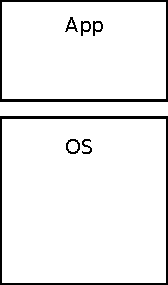
\includegraphics[width=0.4\textwidth]{res/propritary-on-os-base.pdf}
		}
		\only<2>{
			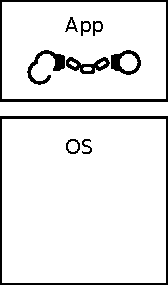
\includegraphics[width=0.4\textwidth]{res/propritary-on-os-app.pdf}
		}
		\only<3>{
			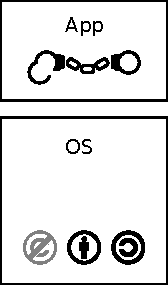
\includegraphics[width=0.4\textwidth]{res/propritary-on-os-all.pdf}
		}
	\end{center}
\end{frame}
\note
{
	\begin{itemize}
		\item proprietäre Applikation auf freiem OS (z.B. Debian GNU/Linux) kein Problem
		\item Open Handcuffs: CC-0 by qubodup https://openclipart.org/detail/171929/open-handcuffs
	\end{itemize}
}

\begin{frame}{Frei mit Proprietär: Library}
	\begin{multicols}{2}
		\begin{center}
			\only<2>{
				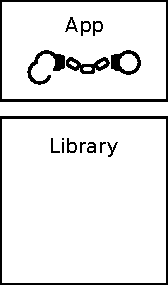
\includegraphics[width=0.4\textwidth]{res/propritary-dynamic-linking-base.pdf}
			}
			\only<3>{
				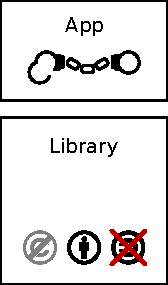
\includegraphics[width=0.4\textwidth]{res/propritary-dynamic-linking-nocopyleft.pdf}
			}
			\only<4->{
				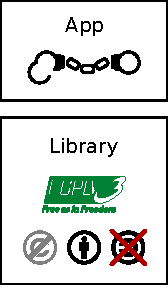
\includegraphics[width=0.4\textwidth]{res/propritary-dynamic-linking-lgpl.pdf}
			}
		\end{center}
		\pagebreak
		\begin{center}
			\only<5>{
				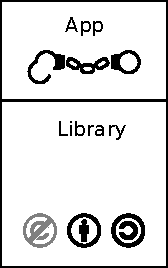
\includegraphics[width=0.4\textwidth]{res/propritary-static-linking-base.pdf}
			}
			\only<6->{
				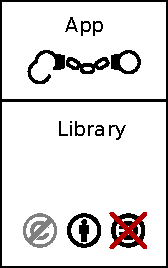
\includegraphics[width=0.4\textwidth]{res/propritary-static-linking-nocopyleft.pdf}
			}
		\end{center}
	\end{multicols}
\end{frame}
\note
{
	\begin{itemize}
		\item dynamisches linken nur gegen Libraries mit Public-Domain, permissiven Lizenzen oder LGPL
		\item statisches linken nur gegen Libraries mit Public-Domain oder permissiven Lizenzen
	\end{itemize}
}

\begin{frame}{Frei mit Proprietär: Code Übernahme}
	\begin{multicols}{2}
		\begin{center}
			\only<2>{
				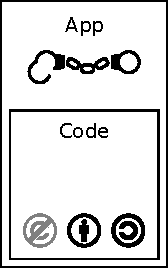
\includegraphics[width=0.4\textwidth]{res/propritary-use-code-base.pdf}
			}
			\only<3->{
				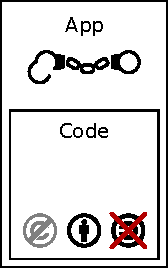
\includegraphics[width=0.4\textwidth]{res/propritary-use-code-nocopyleft.pdf}
			}
		\end{center}
		\pagebreak
		\begin{center}
			\only<4>{
				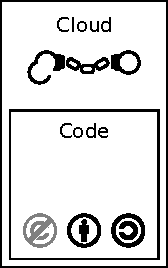
\includegraphics[width=0.4\textwidth]{res/propritary-cloud-base.pdf}
			}
			\only<5->{
				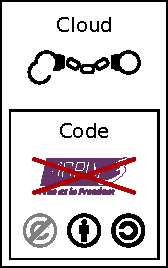
\includegraphics[width=0.4\textwidth]{res/propritary-cloud-agpl.pdf}
			}
		\end{center}
	\end{multicols}
\end{frame}
\note
{
	\begin{itemize}
		\item Verwenden in proprietärem Code: nur Public-Domain oder permissive Lizenzen
		\item Code unter Copyleft darf nicht in proprietärer Applikation verwendet werden\footnote{ausser wenn ausschliesslich intern gebraucht, dann ist es Freie Software}
	\end{itemize}
}

\begin{frame}{Verwendung mit Freier Software}
	\begin{itemize}
		\item Patches unter gleicher Lizenz
		\item Lizenz Kompatibilität beachten
	\end{itemize}
	\begin{center}
		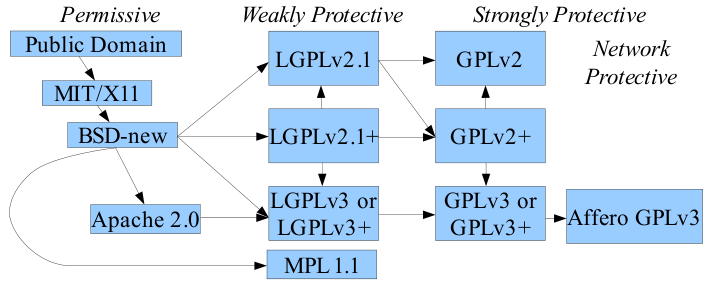
\includegraphics[width=\textwidth]{res/floss-license-compability.png}
	\end{center}
\end{frame}

\begin{frame}{Auswahl einer Lizenz}
	\begin{center}
		\begin{tabular}{ccc}
		
\includegraphics[width=1cm]{res/PD-icon.pdf} & 
\includegraphics[width=1cm]{res/by.pdf} & 
\includegraphics[width=1cm]{res/copyleft.pdf} \\ 
		Public Domain & Permissiv & Copyleft \\
		
\includegraphics[width=2.8cm]{res/cc-zero.pdf} & 
\includegraphics[width=2.8cm]{res/mit-logo.pdf} & 
\includegraphics[width=2.8cm]{res/gpl-v3-logo.pdf} \\
		\hspace{0.3\textwidth} & \hspace{0.3\textwidth} & \hspace{0.3\textwidth} \\
		\end{tabular} 
	\end{center}
	\begin{itemize}
		\item \url{http://choosealicense.com/}
	\end{itemize}
	\vspace{1cm}
\end{frame}
\note
{
	\begin{itemize}
		\item Was will man schützen?
		\item Was will man erlauben?
		\item Was will man verhindern?
	\end{itemize}
}

\begin{frame}{Deklaration der Lizenz}
	\only<beamer:0|handout:1>
	{
	\begin{itemize}
		\item im Projekt (COPYING)
		\item in den Files (SPDX)
		\item in dem Binary (Inkscape)
		\item Keine Lizenz: Code darf nicht benutzt werden
	\end{itemize}
	}
	\begin{center}
		\only<2|handout:2>
		{
			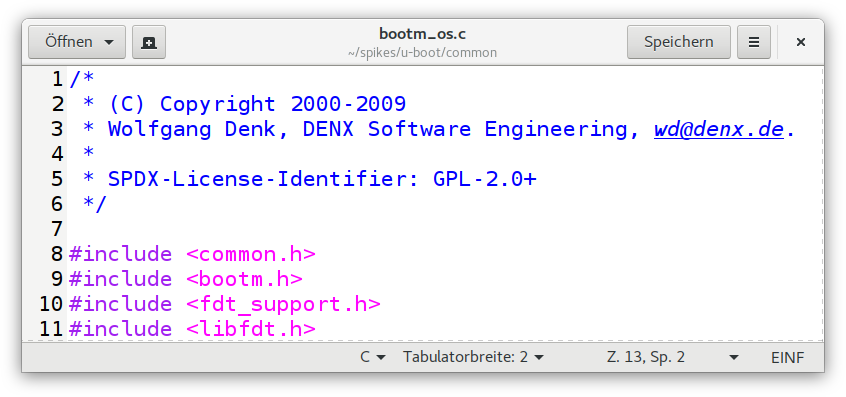
\includegraphics[width=\textwidth]{res/lizenz-source.png}
		}
		\only<3|handout:3>
		{
			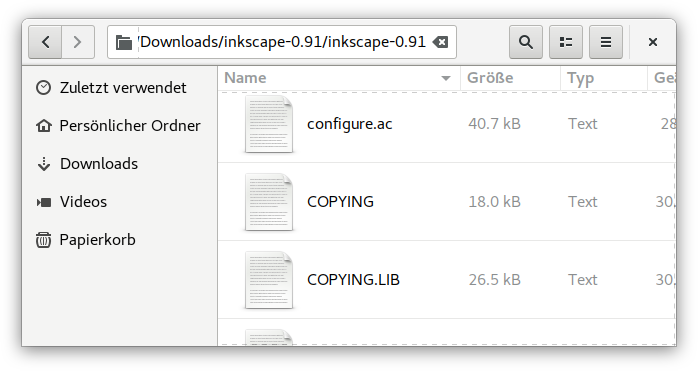
\includegraphics[width=\textwidth]{res/lizenz-file.png}
		}
		\only<4|handout:4>
		{
			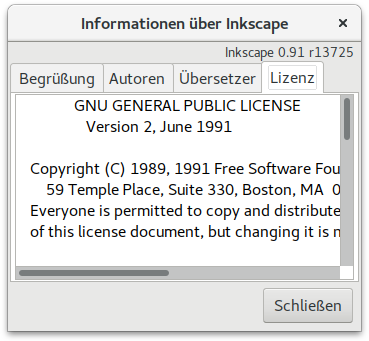
\includegraphics[height=6cm]{res/lizenz-binary.png}
		}
	\end{center}
\end{frame}
\note
{
	\begin{itemize}
		\item im Projekt (COPYING)
		\item in den Files (SPDX)
		\item in dem Binary (Inkscape)
		\item Keine Lizenz: Code darf nicht benutzt werden
	\end{itemize}
}

\begin{frame}{Veröffentlichen der Sourcen}
	\only<2|handout:1>{
		\begin{center}
			\makebox[\textwidth]{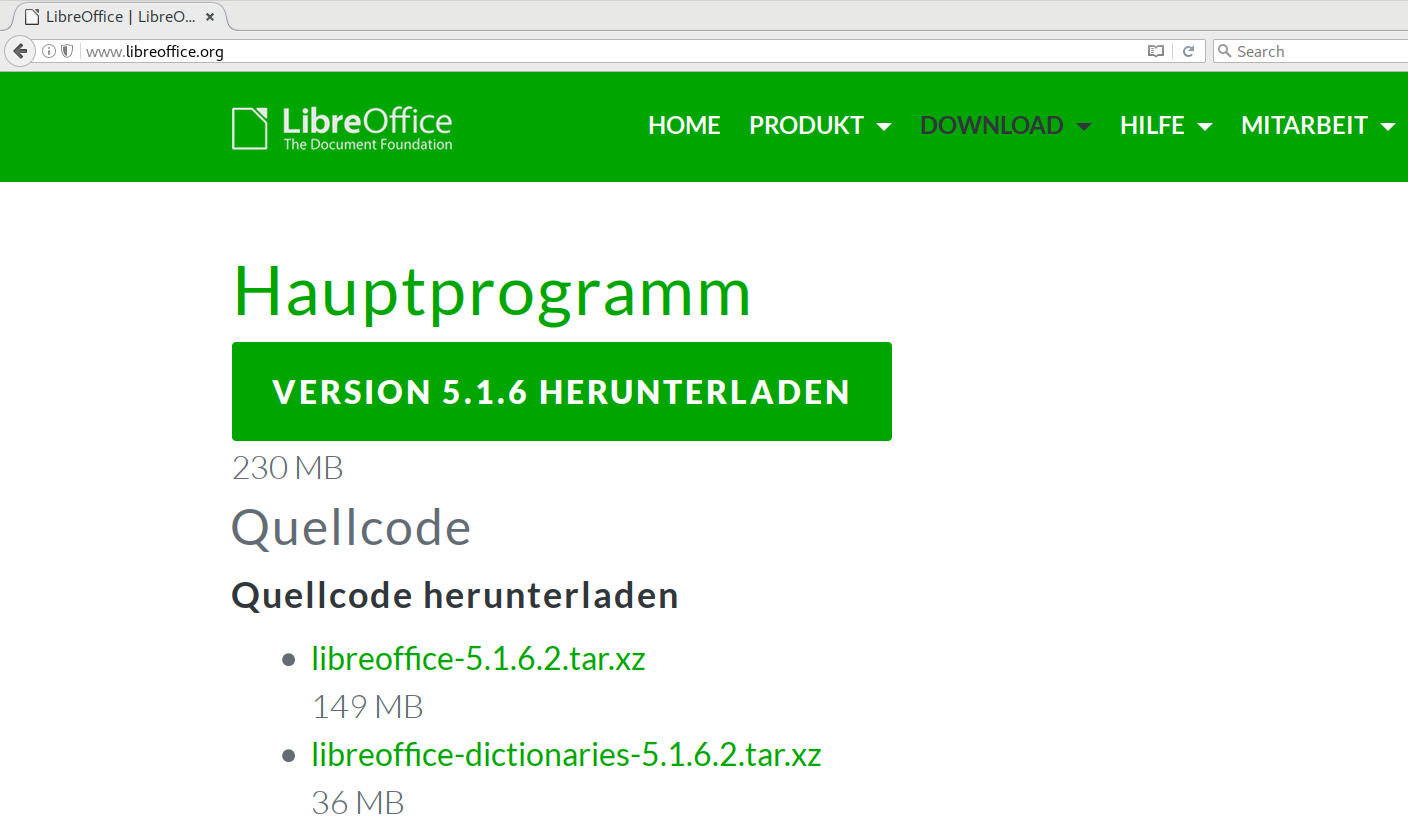
\includegraphics[width=0.98\paperwidth]{res/source-download.png}}
		\end{center}
	}
	\only<3|handout:2>{
		\begin{center}
			\makebox[\textwidth]{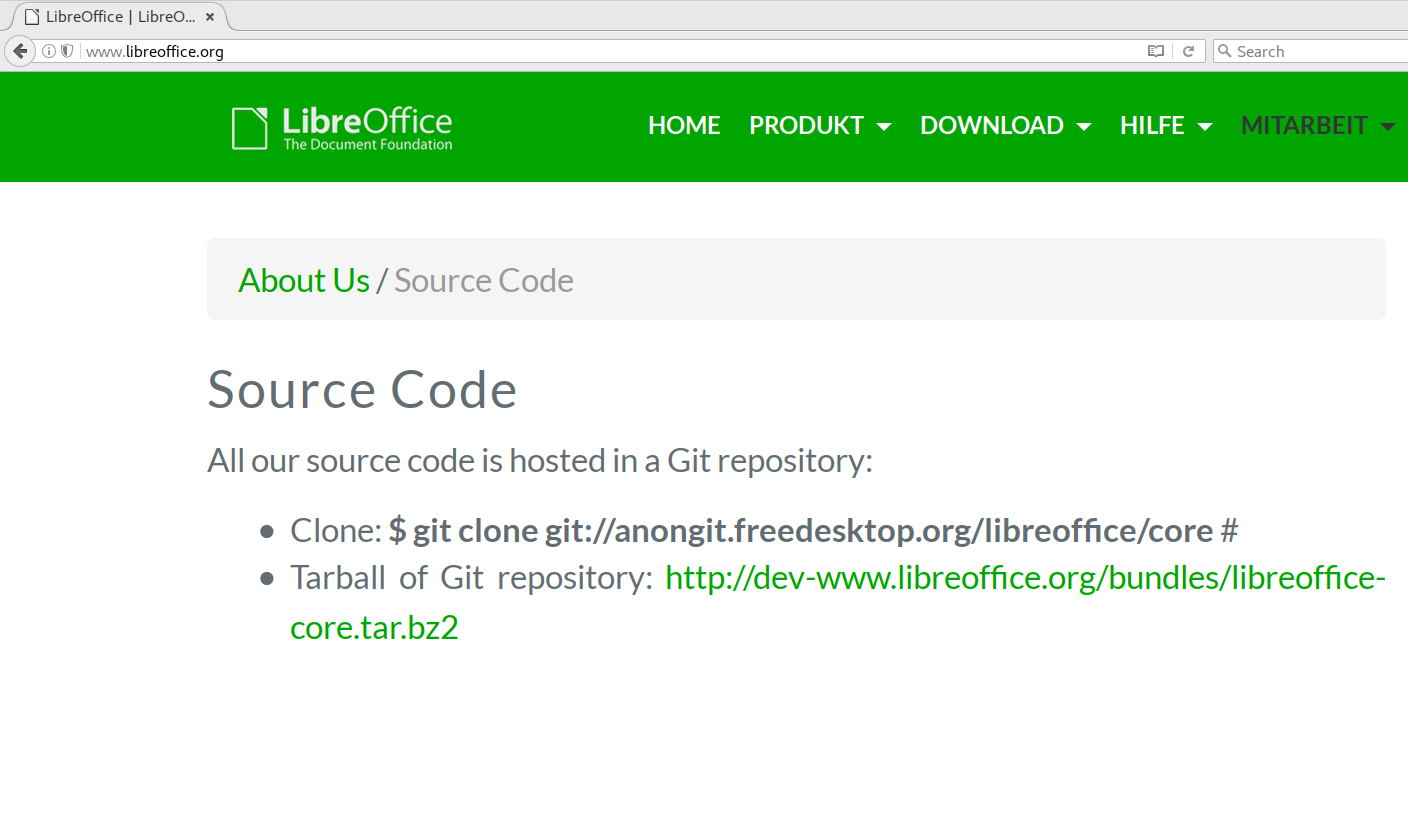
\includegraphics[width=0.98\paperwidth]{res/source-git.png}}
		\end{center}
	}
\end{frame}

\begin{frame}{Verteidigung des eigenen Codes}
	\begin{itemize}
		\item Dialog suchen
		\item \url{http://gpl-violations.org}
	\end{itemize}
\end{frame}
\note
{
  \url{https://en.wikipedia.org/wiki/Gpl-violations.org}
}
